% Asset ID: AS1TrigonometricRatiosTIKZ-003
% Source: P1-Chp9 p.9
% Related section: Bearings
% Purpose: Bearing setup and included angle
\documentclass[tikz,border=8pt]{standalone}
\usepackage{amsmath}
\usetikzlibrary{angles,quotes,calc,arrows.meta}
\begin{document}
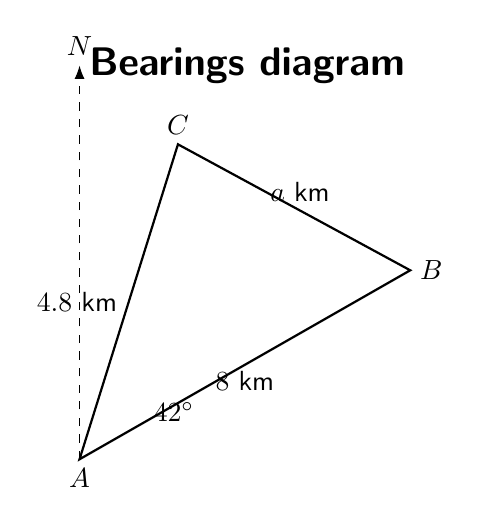
\begin{tikzpicture}[scale=1.0, every node/.style={font=\sffamily}]
\node[font=\sffamily\bfseries\Large, anchor=west] at (0,5) {Bearings diagram};
\coordinate (A) at (0,0);\coordinate (B) at (4.2,2.4);\coordinate (C) at (1.25,4);\draw[dashed,-{Latex}] (A)--(0,5);\node[above] at (0,5) {$N$};\draw[thick] (A)--(B)--(C)--cycle;\node[below] at (A) {$A$};\node[right] at (B) {$B$};\node[above] at (C) {$C$};\node at (2.1,1.0) {$8$ km};\node[left] at (.6,2) {$4.8$ km};\node at (2.8,3.4) {$a$ km};\node at (1.2,.6) {$42^\circ$};
\end{tikzpicture}
\end{document}
